\section{Referencia de la Clase Informe\-Cliente}
\label{classInformeCliente}\index{InformeCliente@{InformeCliente}}
Genera un informe utilizando un identificador de cliente.  


{\tt \#include $<$informereferencia.h$>$}

Diagrama de colaboraci\'{o}n para Informe\-Cliente:\begin{figure}[H]
\begin{center}
\leavevmode
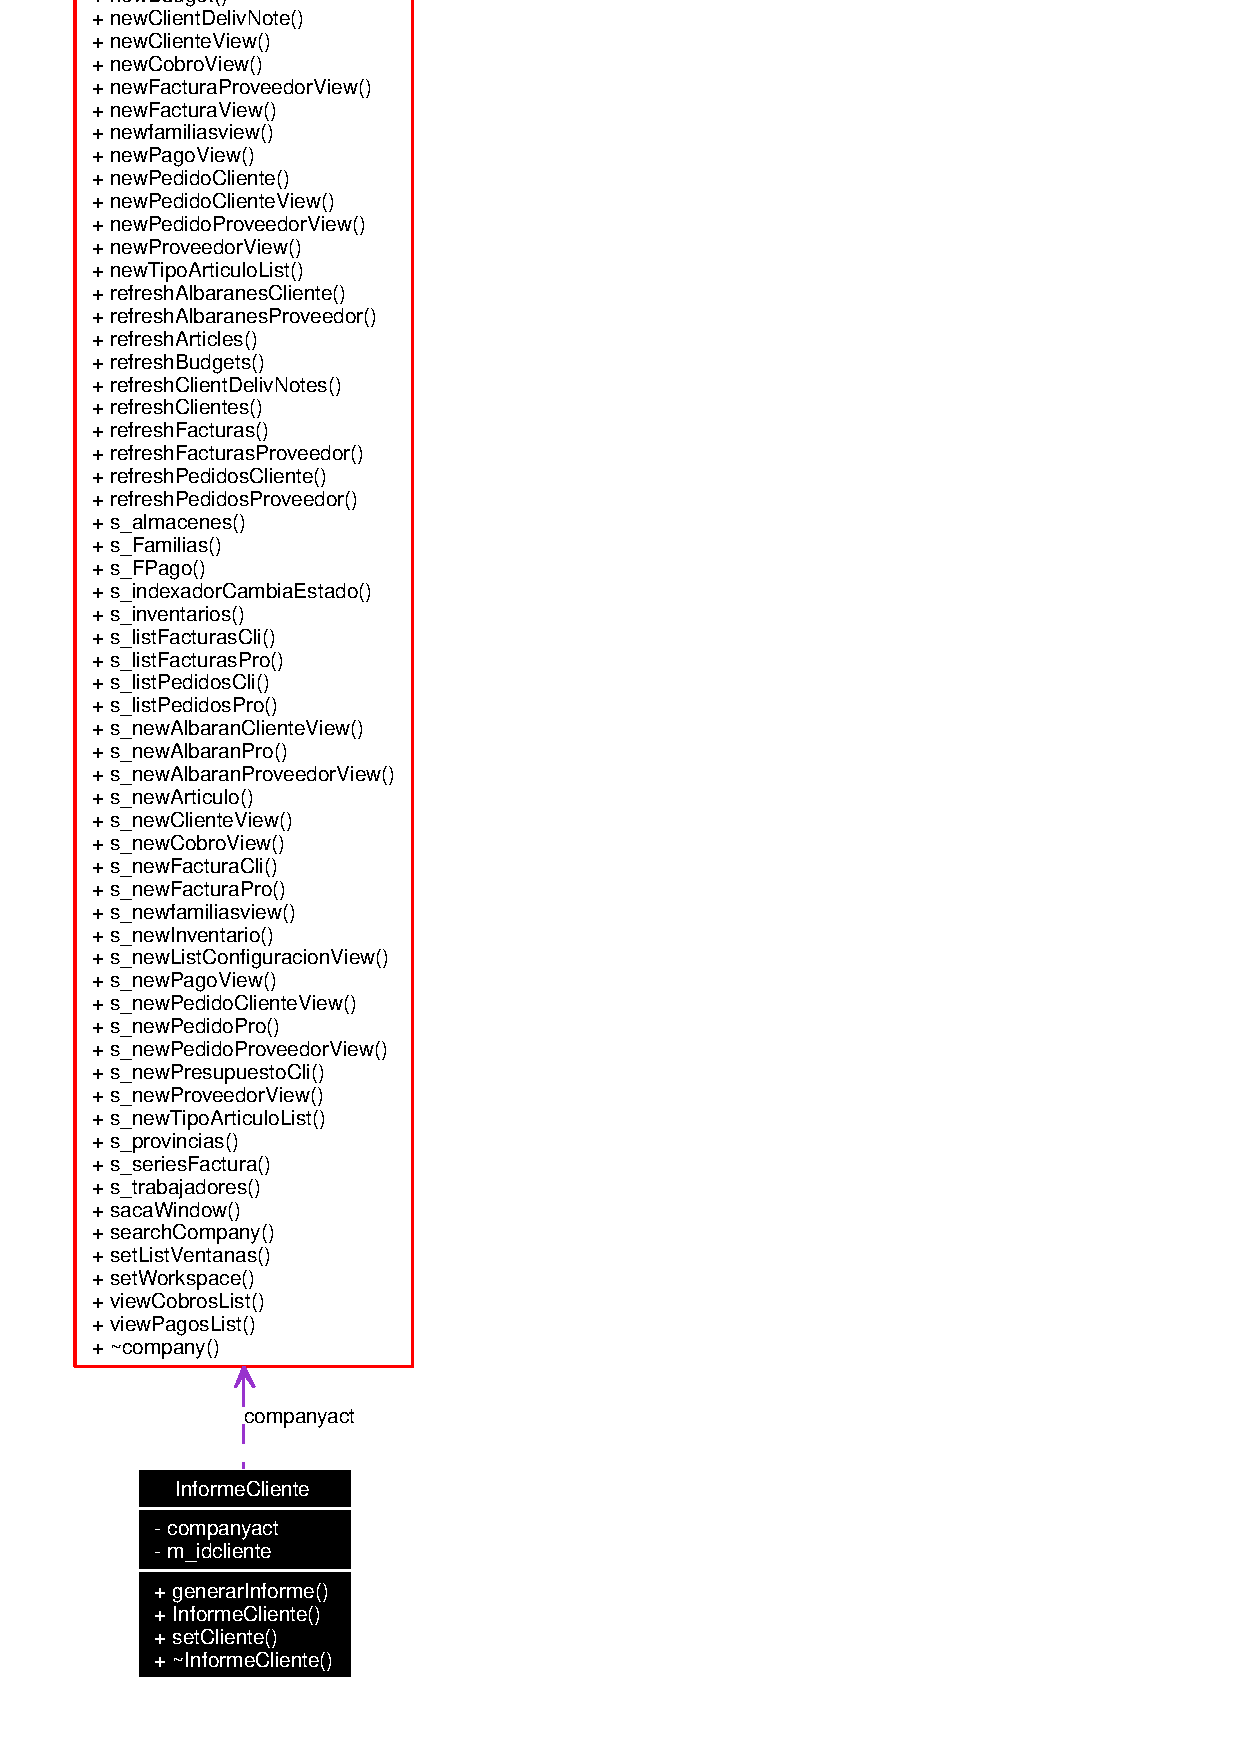
\includegraphics[width=99pt]{classInformeCliente__coll__graph}
\end{center}
\end{figure}
\subsection*{M\'{e}todos p\'{u}blicos}
\begin{CompactItemize}
\item 
void {\bf generar\-Informe} ()
\item 
{\bf Informe\-Cliente} ({\bf company} $\ast$)
\item 
void {\bf set\-Cliente} (QString val)\label{classInformeCliente_a2}

\end{CompactItemize}


\subsection{Descripci\'{o}n detallada}
Genera un informe utilizando un identificador de cliente. 



\subsection{Documentaci\'{o}n del constructor y destructor}
\index{InformeCliente@{Informe\-Cliente}!InformeCliente@{InformeCliente}}
\index{InformeCliente@{InformeCliente}!InformeCliente@{Informe\-Cliente}}
\subsubsection{\setlength{\rightskip}{0pt plus 5cm}Informe\-Cliente::Informe\-Cliente ({\bf company} $\ast$ {\em comp})}\label{classInformeCliente_a1}


================================================================ =================== INFORME CLIENTE ============================ ================================================================ 

\subsection{Documentaci\'{o}n de las funciones miembro}
\index{InformeCliente@{Informe\-Cliente}!generarInforme@{generarInforme}}
\index{generarInforme@{generarInforme}!InformeCliente@{Informe\-Cliente}}
\subsubsection{\setlength{\rightskip}{0pt plus 5cm}void Informe\-Cliente::generar\-Informe ()}\label{classInformeCliente_a0}


Copiamos el archivo.

Copiamos el logo.

Sacamos los datos del cliente

Sacamos todas las referencias de este cliente y las guardamos en el string referencias.

Generacion del informe de ventas.

Generacion del informe de compras.

Generacion del informe de totales de ventas.

Calculo de las cantidades totales en moneda.

Total presupuestado.

Total pedido.

Total trabajado.

Total facturado.

Total cobrado.

Generacion del informe de totales de compras.

Calculo de las cantidades totales en moneda.

Total pedido.

Total trabajado.

Total facturado.

Total cobrado. 

La documentaci\'{o}n para esta clase fu\'{e} generada a partir de los siguientes archivos:\begin{CompactItemize}
\item 
informereferencia.h\item 
informereferencia.cpp\end{CompactItemize}
